\begin{enumerate}[label=\thesection.\arabic*,ref=\thesection.\theenumi]
\item An arch is in the form of a semi-ellipse. It is 8 m wide and 2 m high at the centre. Find the height of the arch at a point 1.5 m from one end.
\label{chapters/11/11/5/4}
\iffalse
\def\mytitle{PYTHON PROGRAMMING ON MATRICES}
\def\myauthor{K.Pavan Kumar}
\def\contact{r170850@rguktrkv.ac.in}
\def\mymodule{Future Wireless Communication (FWC)}
\documentclass[10pt, a4paper]{article}
\usepackage[a4paper,outer=1.5cm,inner=1.5cm,top=1.75cm,bottom=1.5cm]{geometry}
\twocolumn
\usepackage{graphicx}
\graphicspath{{./images/}}
\usepackage[colorlinks,linkcolor={black},citecolor={blue!80!black},urlcolor={blue!80!black}]{hyperref}
\usepackage[parfill]{parskip}
\usepackage{lmodern}
\usepackage{tikz}
	\usepackage{physics}
\usepackage{tabularx}
\usepackage{enumitem}
\usetikzlibrary{calc}
\usepackage{amsmath}
\usepackage{amssymb}
\renewcommand*\familydefault{\sfdefault}
\usepackage{watermark}
\usepackage{lipsum}
\usepackage{xcolor}
\usepackage{listings}
\usepackage{float}
\usepackage{titlesec}
\providecommand{\mtx}[1]{\mathbf{#1}}
\titlespacing{\subsection}{1pt}{\parskip}{3pt}
\titlespacing{\subsubsection}{0pt}{\parskip}{-\parskip}
\titlespacing{\paragraph}{0pt}{\parskip}{\parskip}


\newcommand{\myvec}[1]{\ensuremath{\begin{pmatrix}#1\end{pmatrix}}}
\let\vec\mathbf
\lstset{
frame=single, 
breaklines=true,
columns=fullflexible
}
\thiswatermark{\centering \put(0,-110.0){
\includegraphics[scale=0.3]{logo.png}} }
\title{\mytitle}
\author{\myauthor\hspace{1em}\\\contact\\FWC22011\hspace{6.5em}IITH\hspace{0.5em}\mymodule\hspace{6em}Matrix:conic}
\date{}
\begin{document}
	\maketitle
	\tableofcontents
   \section{Problem}
   \fi
\\
\solution 
	\begin{figure}[!ht]
		\centering
 \includegraphics[width=\columnwidth]{chapters/11/11/5/4/figs/ellipse.png}
		\caption{}
		\label{fig:11/11/5/4}
  	\end{figure}
	\iffalse

\section{Construction}
  \includegraphics[scale=0.45]{ellipse.png}
  	\begin{center}
  Figure of construction
  	\end{center}
  \section{Solution}
Ellipse equation:
\begin{align}
\frac{x^2}{16}+\frac{y^2}{4}=1
\end{align}
The standard equation of the conics is given as :
\begin{align}
\vec{x}^{\top}\vec{V}\vec{x}+2\vec{u}^{\top}\vec{x}+f=0
\label{eq:conic}
\end{align}

The given ellipse can be expressed in  conics as\\ 
\begin{align}
\vec{u} = \myvec{0 \\0} , f =-1 
\end{align}


    The input parameters for this construction are
\begin{center}
\begin{tabular}{|c|c|c|}
	\hline
	\textbf{Symbol}&\textbf{Value}&\textbf{Description}\\
	\hline
	$a$ &4&Length of semi major axis\\
	\hline
    $b$ &2&Length of semi minor axis\\
    \hline
    $\vec{e_1}$ &\myvec{1\\0}&Standard basis vector along X-axis \\
	\hline
    $\vec{m}$ & $\myvec{0\\1}$ &Directional vector along Y-axis\\
	\hline
\end{tabular}


    The steps for constructing above figure are :
\begin{enumerate}
 \item Generate semi-ellipse with semi major axis and semi minor axis lengths equal to $\vec{a}$ and $\vec{b}$ respectively.
 \item Locate center $\vec{c}$ and vertices $\vec{A_1}$ and $\vec{A_2}$.
 \item Locate point $\vec{q}$ on the major axis.
 \item Find the height of ellipse at $\vec{q}$ .
\end{enumerate}

For the standard ellipse, the length of the major axis and minor axis are:
\begin{align}
2\sqrt{\abs{\frac{f_0}{\lambda_1}}} \\
2\sqrt{\abs{\frac{f_0}{\lambda_2}}} 
\end{align}

Given ,The major axis and minor axis are 8m and 4m in length respectively. \\
$*f_0=\vec{u}^{\top} \vec{v}^{-1}\vec{u}-f=1$ 


Equation (5)$\implies2\sqrt{\abs{\frac{f_0}{\lambda_1}}}$=8\\
$\implies\lambda_1$=1/16

Equation (6)$\implies2\sqrt{\abs{\frac{f_0}{\lambda_2}}}$=4\\
$\implies\lambda_2$=1/4

\begin{align}
   \implies \vec{v}=\myvec{\lambda_1&0\\0&\lambda_2}=\myvec{1/16&0\\0&1/4}
\end{align}


\textbf{vertices:}            $\vec{v}=\pm a\vec{e_1}$
\begin{align}
\vec{v}=\pm a\myvec{1\\0} =\pm\myvec{4\\0}\\
Let, \vec{A_1}=\myvec{4 \\0},\vec{A_2}=\myvec{-4 \\0}
\end{align}


 To find the height of ellipse at a point 1.5m from end,
 \begin{align}
\implies\norm{\vec{A_1}-\vec{q}}^2 = (1.5)^2 \\
(\vec{A_1}-\vec{q})^\top(\vec{A_1}-\vec{q})=(1.5)^2\\
\norm{\vec{A_1}^2}+\norm{\vec{q}^2}-2\vec{A_1}^{\top}\vec{q}=(1.5)^2\\
\norm{\vec{q}}^2-2\vec{A}^\top\vec{q}+13.75=0\\
 \vec{e_2}^\top\vec{q}=0 \\
 \implies \vec{q}=\lambda\vec{e_1} 
\end{align}
substitute (14) in (12);
$\implies \lambda^2-8\lambda+13.75=0$\\
$\implies\lambda=\frac{5}{2},\frac{11}{2}$\\
The length of semi major axis is 4m,we need to find height of ellipse at a point 1.5m from one end.
\\$\therefore$ the possible solution  is $\lambda=\frac{5}{2}$
\\$\lambda$ lies on x-axis.
 \begin{align} 
\implies \vec{q}=\myvec{\frac{5}{2}\\0}
\end{align}



\textbf{Directional vector m:}\\
The unit vector along $\vec{Y}$-axis become the directional vector along $\vec{Y}$-axis.
\begin{align}
    \implies\vec{m}=\myvec{0\\1}
\end{align}

\end{center}
\textbf{Theorem:}
The points of intersection of the line 
\begin{align}
L: \quad \vec{x} = \vec{q} + \mu \vec{m} \quad \mu \in \mathbb{R}
\end{align}
with the conic section in \eqref{eq:conic} are given by
\begin{align}
\vec{x}_i = \vec{q} + \mu_i \vec{m}
\end{align}

where $\mu_i$ is given by  \\
\begin{align}
\mu_i =\frac{1}
{\vec{m}^{\top}\vec{V}\vec{m}}
\left(-\vec{m}^{\top}(\vec{V}\vec{q}+\vec{u}) \pm Z\right) 
\end{align}
\\
\\
 Z = $\sqrt{[\vec{m}^{\top}(\vec{V}\vec{q}+\vec{u})]^2 -(\vec{q}^{\top}\vec{V}\vec{q} + 2\vec{u}^{\top}\vec{q} +f)(\vec{m}^{\top}\vec{V}\vec{m})}$
 \\
 \\

By substituting the vectors $\vec{m}$,$\vec{q}$,$\vec{v}$,$\vec{u}$ and constant f in  (19) results intersection points on the conic section .Consider absolute value ,say $\vec{H}$.

 $\vec{H}$ gives height of ellipse at point $\vec{q}$.

\begin{center}
    (or)
\end{center}
        
 $\norm{\vec{H}-\vec{q}}$ results the same.\\
  $\therefore$ Height of ellipse at $\vec{q}$=1.56.

\textbf{termux commands :}
\begin{lstlisting}
bash conic.sh............using shell command
\end{lstlisting}

\begin{center}
Below python code realizes the above construction :
\fbox{\parbox{8.5cm}{\url{https://github.com/FWC_module1/blob/main/matrices/conic/conic.py}}}
\end{center}
\end{document}
\fi

\item A rod of length 12cm moves with its ends always touching the coordinate axes. Determine the equation of locus of a point  P on the rod, which is 3cm from the end in contact with $x-axis$.
\label{chapters/11/11/5/5}
\iffalse
\documentclass[journal,11pt,twocolumn]{IEEEtran}
%
\usepackage{setspace}
\usepackage{gensymb}
%\doublespacing
\singlespacing

%\usepackage{graphicx}
%\usepackage{amssymb}
%\usepackage{relsize}
\usepackage[cmex10]{amsmath}
%\usepackage{amsthm}
%\interdisplaylinepenalty=2500
%\savesymbol{iint}
%\usepackage{txfonts}
%\restoresymbol{TXF}{iint}
%\usepackage{wasysym}
\usepackage{amsthm}
%\usepackage{iithtlc}
\usepackage{mathrsfs}
\usepackage{txfonts}
\usepackage{stfloats}
\usepackage{bm}
\usepackage{cite}
\usepackage{cases}
\usepackage{subfig}
%\usepackage{xtab}
\usepackage{longtable}
\usepackage{multirow}
%\usepackage{algorithm}
%\usepackage{algpseudocode}
\usepackage{enumitem}
\usepackage{mathtools}
\usepackage{steinmetz}
\usepackage{tikz}
\usepackage{circuitikz}
\usepackage{verbatim}
\usepackage{tfrupee}
\usepackage[breaklinks=true]{hyperref}
%\usepackage{stmaryrd}
\usepackage{tkz-euclide} % loads  TikZ and tkz-base
%\usetkzobj{all}
\usetikzlibrary{calc,math}
\usepackage{listings}
    \usepackage{color}                                            %%
    \usepackage{array}                                            %%
    \usepackage{longtable}                                        %%
    \usepackage{calc}                                             %%
    \usepackage{multirow}                                         %%
    \usepackage{hhline}                                           %%
    \usepackage{ifthen}                                           %%
  %optionally (for landscape tables embedded in another document): %%
    \usepackage{lscape}     
\usepackage{multicol}
\usepackage{chngcntr}
%\usepackage{enumerate}

%\usepackage{wasysym}
%\newcounter{MYtempeqncnt}
\DeclareMathOperator*{\Res}{Res}
%\renewcommand{\baselinestretch}{2}
\renewcommand\thesection{\arabic{section}}
\renewcommand\thesubsection{\thesection.\arabic{subsection}}
\renewcommand\thesubsubsection{\thesubsection.\arabic{subsubsection}}

\renewcommand\thesectiondis{\arabic{section}}
\renewcommand\thesubsectiondis{\thesectiondis.\arabic{subsection}}
\renewcommand\thesubsubsectiondis{\thesubsectiondis.\arabic{subsubsection}}

% correct bad hyphenation here
\hyphenation{op-tical net-works semi-conduc-tor}
\def\inputGnumericTable{}                                 %%

\lstset{
%language=C,
frame=single, 
breaklines=true,
columns=fullflexible
}
%\lstset{
%language=tex,
%frame=single, 
%breaklines=true
%}

\begin{document}
%


\newtheorem{theorem}{Theorem}[section]
\newtheorem{problem}{Problem}
\newtheorem{proposition}{Proposition}[section]
\newtheorem{lemma}{Lemma}[section]
\newtheorem{corollary}[theorem]{Corollary}
\newtheorem{example}{Example}[section]
\newtheorem{definition}[problem]{Definition}
%\newtheorem{thm}{Theorem}[section] 
%\newtheorem{defn}[thm]{Definition}
%\newtheorem{algorithm}{Algorithm}[section]
%\newtheorem{cor}{Corollary}
\newcommand{\BEQA}{\begin{eqnarray}}
\newcommand{\EEQA}{\end{eqnarray}}
\newcommand{\define}{\stackrel{\triangle}{=}}

\bibliographystyle{IEEEtran}
%\bibliographystyle{ieeetr}


\providecommand{\mbf}{\mathbf}
\providecommand{\pr}[1]{\ensuremath{\Pr\left(#1\right)}}
\providecommand{\qfunc}[1]{\ensuremath{Q\left(#1\right)}}
\providecommand{\sbrak}[1]{\ensuremath{{}\left[#1\right]}}
\providecommand{\lsbrak}[1]{\ensuremath{{}\left[#1\right.}}
\providecommand{\rsbrak}[1]{\ensuremath{{}\left.#1\right]}}
\providecommand{\brak}[1]{\ensuremath{\left(#1\right)}}
\providecommand{\lbrak}[1]{\ensuremath{\left(#1\right.}}
\providecommand{\rbrak}[1]{\ensuremath{\left.#1\right)}}
\providecommand{\cbrak}[1]{\ensuremath{\left\{#1\right\}}}
\providecommand{\lcbrak}[1]{\ensuremath{\left\{#1\right.}}
\providecommand{\rcbrak}[1]{\ensuremath{\left.#1\right\}}}
\theoremstyle{remark}
\newtheorem{rem}{Remark}
\newcommand{\sgn}{\mathop{\mathrm{sgn}}}
\providecommand{\abs}[1]{\left\vert#1\right\vert}
\providecommand{\res}[1]{\Res\displaylimits_{#1}} 
\providecommand{\norm}[1]{\left\lVert#1\right\rVert}
%\providecommand{\norm}[1]{\lVert#1\rVert}
\providecommand{\mtx}[1]{\mathbf{#1}}
\providecommand{\mean}[1]{E\left[ #1 \right]}
\providecommand{\fourier}{\overset{\mathcal{F}}{ \rightleftharpoons}}
%\providecommand{\hilbert}{\overset{\mathcal{H}}{ \rightleftharpoons}}
\providecommand{\system}{\overset{\mathcal{H}}{ \longleftrightarrow}}
	%\newcommand{\solution}[2]{\textbf{Solution:}{#1}}
\newcommand{\solution}{\noindent \textbf{Solution: }}
\newcommand{\cosec}{\,\text{cosec}\,}
\providecommand{\dec}[2]{\ensuremath{\overset{#1}{\underset{#2}{\gtrless}}}}
\newcommand{\myvec}[1]{\ensuremath{\begin{pmatrix}#1\end{pmatrix}}}
\newcommand{\mydet}[1]{\ensuremath{\begin{vmatrix}#1\end{vmatrix}}}
%\numberwithin{equation}{section}
\numberwithin{equation}{subsection}
%\numberwithin{problem}{section}
%\numberwithin{definition}{section}
\makeatletter
\@addtoreset{figure}{problem}
\makeatother

\let\StandardTheFigure\thefigure
\let\vec\mathbf
%\renewcommand{\thefigure}{\theproblem.\arabic{figure}}
\renewcommand{\thefigure}{\theproblem}
%\setlist[enumerate,1]{before=\renewcommand\theequation{\theenumi.\arabic{equation}}
%\counterwithin{equation}{enumi}


%\renewcommand{\theequation}{\arabic{subsection}.\arabic{equation}}

\def\putbox#1#2#3{\makebox[0in][l]{\makebox[#1][l]{}\raisebox{\baselineskip}[0in][0in]{\raisebox{#2}[0in][0in]{#3}}}}
     \def\rightbox#1{\makebox[0in][r]{#1}}
     \def\centbox#1{\makebox[0in]{#1}}
     \def\topbox#1{\raisebox{-\baselineskip}[0in][0in]{#1}}
     \def\midbox#1{\raisebox{-0.5\baselineskip}[0in][0in]{#1}}

\vspace{3cm}


\title{Que: 11.11.5.5}
\author{Nikam Pratik Balasaheb (EE21BTECH11037)}





% make the title area
\maketitle

\newpage

%\tableofcontents

\bigskip

\renewcommand{\thefigure}{\theenumi}
\renewcommand{\thetable}{\theenumi}
%\renewcommand{\theequation}{\theenumi}

\section{Problem}


\section{Solution}
\fi
Let the angle made by the rod with x-axis be $\theta$.  Then
\begin{enumerate}

\item x-intercept:
	\begin{align}
	\vec{A} = \myvec{12\cos{\theta}\\0}
	\end{align}

\item y-intercept:
	\begin{align}
		\vec{B} =\myvec{0\\12\sin{\theta}}
	\end{align}

\item direction vector of rod:
	\begin{align}
		\vec{A}-\vec{B} = 12\myvec{\cos{\theta} \\ -\sin{\theta}}
	\end{align}
	Unit vector along direction vector:
	\begin{align}
		\vec{m} = \myvec{\cos{\theta} \\ -\sin{\theta}}
	\end{align}

\item given point $\vec{P}$:
	\begin{align}
		\vec{P} &= \vec{A} - 3 \vec{m}\\
			&= \myvec{9 \cos{\theta} \\ 3 \sin{\theta}}
	\end{align}
\item parametric form of locus:
	\begin{align}
		\vec{x} = \myvec{9\cos{\theta} \\ 3\sin{\theta}}\\
	\end{align}
	Consider $\vec{Q} = \myvec{\frac{1}{9}&0\\0&\frac{1}{3}}$
	\begin{align}
		\vec{Q}\vec{x} &= \myvec{\cos{\theta}\\ \sin{\theta}}\\
		\norm{\vec{Q}\vec{x}}^2 &= 1\\
		\brak{\vec{Q}\vec{x}}^{\top} \brak{\vec{Q}\vec{x}} &= 1\\
		\vec{x}^{\top}\vec{Q}^{\top}\vec{Q}\vec{x} &= 1\\
		\vec{x}^T\myvec{\frac{1}{81} & 0 \\ 0 & \frac{1}{9}} \vec{x} &= 1
	\end{align}
	The locus of point $\vec{P}$ is a conic 
	\begin{align}\vec{x}^{\top} \vec{V} \vec{x} + 2 \vec{u}^{\top} \vec{x} +f= 0
	\end{align}
	where,
	\begin{align}
		\vec{V} &= \myvec{\frac{1}{81}&0\\0&\frac{1}{9}}\\
		\vec{u} &= \myvec{0\\0}\\
		f &= -1
	\end{align}
\end{enumerate}
See Table 
	\ref{tab:chapters/11/11/5/5/}.
\begin{table}[h!]
	\begin{center}
		%%%%%%%%%%%%%%%%%%%%%%%%%%%%%%%%%%%%%%%%%%%%%%%%%%%%%%%%%%%%%%%%%%%%%%
%%                                                                  %%
%%  This is a LaTeX2e table fragment exported from Gnumeric.        %%
%%                                                                  %%
%%%%%%%%%%%%%%%%%%%%%%%%%%%%%%%%%%%%%%%%%%%%%%%%%%%%%%%%%%%%%%%%%%%%%%

\begin{tabular}[]{|c|c|c|}
\hline
Parameter	& Value	& Description \\ \hline
$\vec{A}$	& $\myvec{12 \cos{\theta}\\0}$ & x-intercept of rod \\ \hline
$\vec{C}$	& $\myvec{0\\ 12 \sin{\theta}}$ & y-intercept of the rod\\ \hline
$\vec{P}$	& $\myvec{9 \cos{\theta} \\ 3\sin{\theta}}  $ & Point on rod, at given distance from $\vec{A} $ \\ \hline
$\theta$ 		& $\frac{\pi}{3}$ & parameter $\theta$ for $\vec{A}, \vec{B},\vec{P}$\\[1pt] \hline
length	& 12 	& Length of the rod \\ \hline
dist	& 3	& Distance between $\vec{A}, \vec{P}$\\ \hline
\end{tabular}

	\end{center}
	\caption{}
	\label{tab:chapters/11/11/5/5/}
\end{table}
See Fig.
    \ref{fig:chapters/11/11/5/5/}
\begin{figure}[h!]
  \centering
    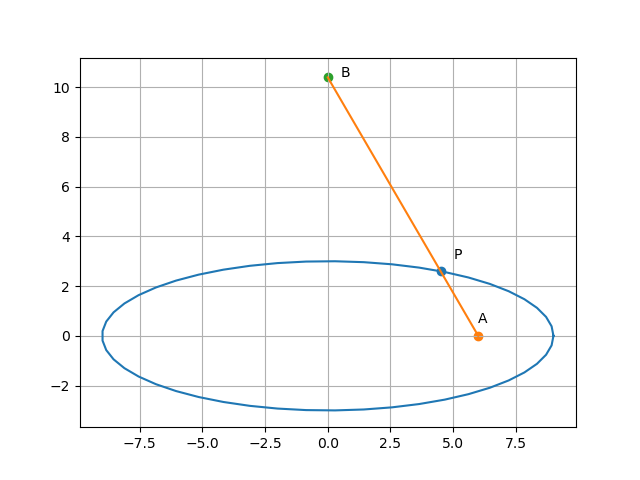
\includegraphics[width=\columnwidth]{chapters/11/11/5/5/figs/Figure_1.png}
    \caption{}
    \label{fig:chapters/11/11/5/5/}
\end{figure}





\item A man running a racecourse notes that the sum of the distances from the two flag posts from him is always 10 m and the distance between the flag posts is 8 m. Find the equation of the posts traced by the man. 
\label{chapters/11/11/5/7}
\iffalse
\documentclass[12pt]{article}
\usepackage{graphicx}
\usepackage[none]{hyphenat}
\usepackage{graphicx}
\usepackage{listings}
\usepackage[english]{babel}
\usepackage{graphicx}
\usepackage{caption} 
\usepackage{booktabs}
\usepackage{array}
\usepackage{amssymb} % for \because
\usepackage{amsmath}   % for having text in math mode
\usepackage{extarrows} % for Row operations arrows
\usepackage{listings}
\lstset{
  frame=single,
  breaklines=true
}
\usepackage{hyperref}
  
%Following 2 lines were added to remove the blank page at the beginning
\usepackage{atbegshi}% http://ctan.org/pkg/atbegshi
\AtBeginDocument{\AtBeginShipoutNext{\AtBeginShipoutDiscard}}


%New macro definitions
\newcommand{\mydet}[1]{\ensuremath{\begin{vmatrix}#1\end{vmatrix}}}
\providecommand{\brak}[1]{\ensuremath{\left(#1\right)}}
\providecommand{\norm}[1]{\left\lVert#1\right\rVert}
\providecommand{\abs}[1]{\left\vert#1\right\vert}
\newcommand{\solution}{\noindent \textbf{Solution: }}
\newcommand{\myvec}[1]{\ensuremath{\begin{pmatrix}#1\end{pmatrix}}}
\let\vec\mathbf


\begin{document}

\begin{center}
\title{\textbf{Conic Sections - Ellipse}}
\date{\vspace{-5ex}} %Not to print date automatically
\maketitle
\end{center}
\setcounter{page}{1}

\section{11$^{th}$ Maths - Chapter 11}
This is Problem-7 from Exercise 11.5
\begin{enumerate}

\solution 
\fi
The conic section for the given problem is an ellipse. Let $\vec{O}\myvec{0 \\ 0}$ be the centre of the Ellipse. Then, the focii are given by 
\begin{align}
    \label{eq:chapters/11/11/5/7/ellipseEq1}
	\vec{F_1} = \myvec{ 4 \\ 0} \\
	\vec{F_2} = \myvec{ -4 \\ 0} 
\end{align}
The sum of the distances from two focii to the point on the locus of the ellipse is equal to $10m$. Let $\vec{P}\myvec{p \\ 0 }$ and $\vec{Q}\myvec{-q \\ 0}$ be the vertices of the ellipse. Then
\begin{align}
	\norm{\vec{P}-\vec{F_1}} + \norm{\vec{P}-\vec{F_2}} = 10 \\
         \brak{p-4} + \brak{p+4} = 10 \\
	 2p = 10 \\
	 p = 5  \\
	 \therefore \vec{P} = \myvec{5 \\ 0}
\end{align}
Similarly
\begin{align}
	\norm{\vec{Q}-\vec{F_1}} + \norm{\vec{Q}-\vec{F_2}} = 10 \\
         \brak{q-4} + \brak{q+4} = 10 \\
	 2q = 10 \\
	 q = 5 \\
	 \therefore \vec{Q} = \myvec{-5 \\ 0}
\end{align}
We know that the Vertex of a standard ellipse is given by
\begin{align}
	\vec{P} &=  \myvec{\sqrt{\abs{\frac{f_0}{\lambda_1}}} \\ 0} \\
	\myvec{5 \\ 0} &=  \myvec{\sqrt{\abs{\frac{f_0}{\lambda_1}}} \\ 0} \\
	\frac{f_0}{\lambda_1} &= 25 \\
	\label{eq:chapters/11/11/5/7/eqV}
	f_0 &= 25\lambda_1 
\end{align}
We know that the Focii for standard Ellipse are given as
\begin{align}
	\label{eq:chapters/11/11/5/7/eqV1}
	\vec{F} &= \pm e\sqrt{\frac{\abs{f_0}}{\lambda_2\brak{1-e^2}}}\vec{e}_1
\end{align}
Substituting values of $\vec{F_1}$ from \eqref{eq:chapters/11/11/5/7/ellipseEq1} and $f_0$ from \eqref{eq:chapters/11/11/5/7/eqV}
\begin{align}
	   \label{eq:chapters/11/11/5/7/eqV2}
	   \eqref{eq:chapters/11/11/5/7/eqV1} \implies \myvec{4 \\0}  &=e\sqrt{\frac{25\lambda_1}{\lambda_2\brak{1-e^2}}}\vec{e}_1
\end{align}
We know that 
\begin{align}
	1-e^2 = \frac{\lambda_1}{\lambda_2} \\
	\eqref{eq:chapters/11/11/5/7/eqV2} \implies  4 &= 5e \\
        e &= \frac{4}{5} \\
	\therefore \frac{\lambda_1}{\lambda_2} &= 1 - \brak{\frac{4}{5}}^2 \\
	&= \frac{9}{25} \\
	\vec{n} &= \sqrt{\frac{\lambda_2}{f_0}}\vec{e}_1\\
	 &= \sqrt{\frac{\lambda_2}{25\lambda_1}}\vec{e}_1\\
	 &= \frac{1}{5} \times \frac{5}{3}\vec{e}_1\\
	 &= \frac{1}{3}\vec{e}_1 \\
	 c &= \frac{1}{e\sqrt{1-e^2}} = \frac{25}{12}
\end{align}
For the standard ellipse, $f$ is given as 
\begin{align}
	\label{eq:chapters/11/11/5/7/eqV3}
	f &= \norm{\vec{n}}^2 \norm{\vec{F}}^2 - c^2 e^2 \\
	&= \brak{\frac{1}{3}}^216 - \frac{25}{9} \\
	&= -1 \\
	f_0 &= -f = 1 \\
	\lambda_1 &= \frac{f_0}{25} = \frac{1}{25}\\
	\lambda_2 &= \frac{25\lambda_1}{9} = \frac{1}{9} \\
	\therefore \vec{V} &= \myvec{\lambda_1 & 0 \\ 0 & \lambda_2} = \myvec{\frac{1}{25} & 0 \\ 0 & \frac{1}{9}}
\end{align}
For a standard ellipse, $\vec{u}=0$. 

The generic equation of conic section is given as
\begin{align}
	\label{eq:chapters/11/11/5/7/ellipseEq2}
	g\brak{\vec{x}} &= \vec{x}^T\vec{V}\vec{x} + 2\vec{u}^T\vec{x} + f = 0 \\ 
	&= \vec{x}^T\myvec{\frac{1}{25} & 0 \\ 0 & \frac{1}{9}}\vec{x}- 1  = 0 
\end{align}
The relevant diagram is shown in Figure \ref{fig:chapters/11/11/5/7/Fig1}
\begin{figure}[!h]
	\begin{center}
		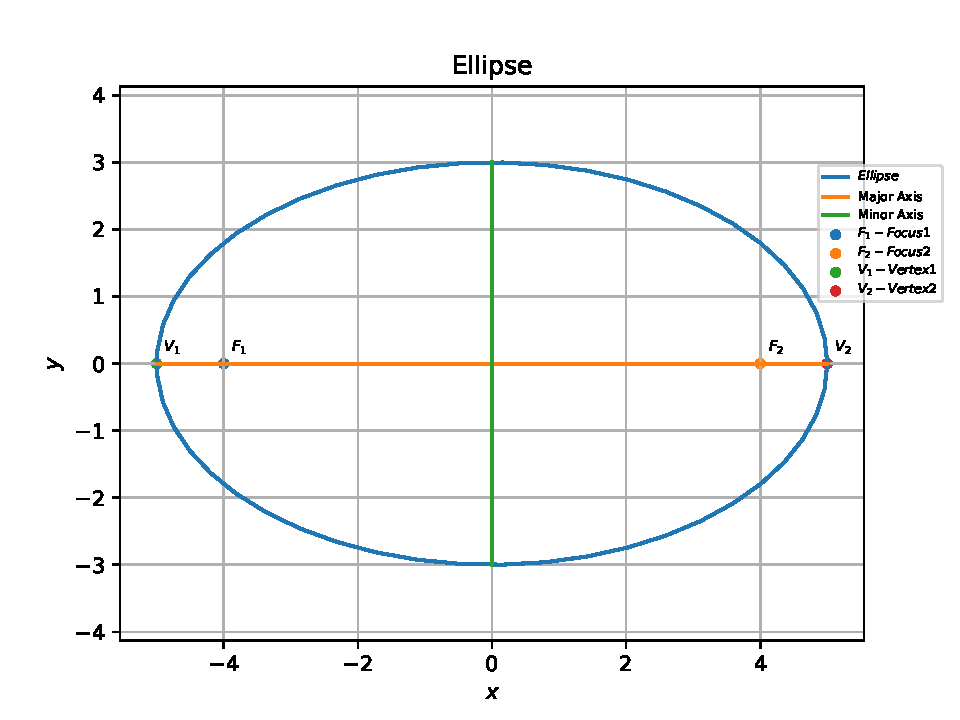
\includegraphics[width=\columnwidth]{chapters/11/11/5/7/figs/problem7.pdf}
	\end{center}
\caption{}
\label{fig:chapters/11/11/5/7/Fig1}
\end{figure}

\end{enumerate}
In each of the following exercises, find the coordinates of the foci, the vertices,the length of major axis, the minor axis,the eccentricity and the length of the latus rectum of the ellipse.
\begin{enumerate}[label=\thesection.\arabic*,ref=\thesection.\theenumi,resume*]
\numberwithin{equation}{enumi}
\numberwithin{figure}{enumi}
\numberwithin{table}{enumi}


  \item $\frac{x^2}{36}+\frac{y^2}{16}=1$
\\
\solution
\iffalse
\documentclass[12pt]{article}
\usepackage{graphicx}
\usepackage[none]{hyphenat}
\usepackage{graphicx}
\usepackage{listings}
\usepackage[english]{babel}
\usepackage{graphicx}
\usepackage{caption} 
\usepackage{booktabs}
\usepackage{array}
\usepackage{amssymb} % for \because
\usepackage{amsmath}   % for having text in math mode
\usepackage{extarrows} % for Row operations arrows
\usepackage{listings}
\lstset{
  frame=single,
  breaklines=true
}
\usepackage{hyperref}
  
%Following 2 lines were added to remove the blank page at the beginning
\usepackage{atbegshi}% http://ctan.org/pkg/atbegshi
\AtBeginDocument{\AtBeginShipoutNext{\AtBeginShipoutDiscard}}


%New macro definitions
\newcommand{\mydet}[1]{\ensuremath{\begin{vmatrix}#1\end{vmatrix}}}
\providecommand{\brak}[1]{\ensuremath{\left(#1\right)}}
\providecommand{\norm}[1]{\left\lVert#1\right\rVert}
\providecommand{\abs}[1]{\left\vert#1\right\vert}
\newcommand{\solution}{\noindent \textbf{Solution: }}
\newcommand{\myvec}[1]{\ensuremath{\begin{pmatrix}#1\end{pmatrix}}}
\let\vec\mathbf


\begin{document}

\begin{center}
\title{\textbf{Conic Sections - Ellipse}}
\date{\vspace{-5ex}} %Not to print date automatically
\maketitle
\end{center}
\setcounter{page}{1}

\section{11$^{th}$ Maths - Chapter 11}
This is Problem-1 from Exercise 11.3
\begin{enumerate}
\item Find the coordinates of the focii, the vertices, the length of major and minor axes, the eccentricity and the length of the latus rectum of an ellipse whose equation is given by $\frac{x^2}{36}+\frac{y^2}{16}=1$.

\solution
\fi
The given equation of ellipse can be rearranged as 
\begin{align}
 4x^2+9y^2-144=0\label{eq:chapters/11/11/3/1/eq1}
\end{align}
The above equation can be equated to the general equation of conic sections
\begin{align}
 g\brak{\vec{x}}=\vec{x}^\top \vec{V} \vec{x} + 2\vec{u}^\top \vec{x} + f = 0\label{eq:chapters/11/11/3/1/eq2}
\end{align}
From \eqref{eq:chapters/11/11/3/1/eq1} and \eqref{eq:chapters/11/11/3/1/eq2}
\begin{align}
 \vec{V} &= \myvec{4&0\\0&9}\label{eq:chapters/11/11/3/1/eq3}\\
 \vec{u} &= \vec{0}\\
 f &= -144
\end{align}
From \eqref{eq:chapters/11/11/3/1/eq3} the eigen values $\lambda_1 \text{ and } \lambda_2$ are given as
\begin{align}
 \lambda_1 &= 4\\
 \lambda_2 &= 9
\end{align}
\begin{enumerate}
\item The eccentricity of the ellipse is given as
\begin{align}
 e &= \sqrt{1 - \frac{\lambda_2}{\lambda_1}} \\
          &= \sqrt{1-\frac{4}{9}}\\
   &= \frac{\sqrt{5}}{3}
\end{align}
\item Finding the coordinates of Focii
\begin{align}
 \vec{F} &= \pm e\sqrt{\frac{\abs{f_0}}{\lambda_2\brak{1-e^2}}}\Vec{e_1}\\
\text{Where }f_0 &=-f\\
 \vec{F} &= \pm2\sqrt{5}\myvec{1\\0}\\
	&= \pm\myvec{2\sqrt{5}\\0}
\end{align}
\item The length of the major axis is given by
\begin{align}
 &2\sqrt{\abs{\frac{f_0}{\lambda_1}}}\\
        &2\sqrt{\abs{\frac{144}{4}}}= 12
\end{align}
\item The length of minor axis is given by
\begin{align}
 &2\sqrt{\abs{\frac{f_0}{\lambda_2}}}\\
        &2\sqrt{\abs{\frac{144}{9}}}= 8
\end{align}
\item The vertices of the ellipse are given by
\begin{align}
 \pm \myvec{0\\\sqrt{\abs{\frac{f_0}{\lambda_2}}}}= \pm \myvec{0\\4}
\end{align}
\item The length of latus rectum is given as
\begin{align}
 &2\frac{\sqrt{\abs{f_0 \lambda_1}}}{\lambda_2} \\
 &= 2\frac{\sqrt{\abs{144\brak{4}}}}{9}\\
 &= \frac{16}{3}
\end{align}
See Fig. 
\ref{fig:chapters/11/11/3/1/Fig1}.
\begin{figure}[!h]
	\begin{center}
		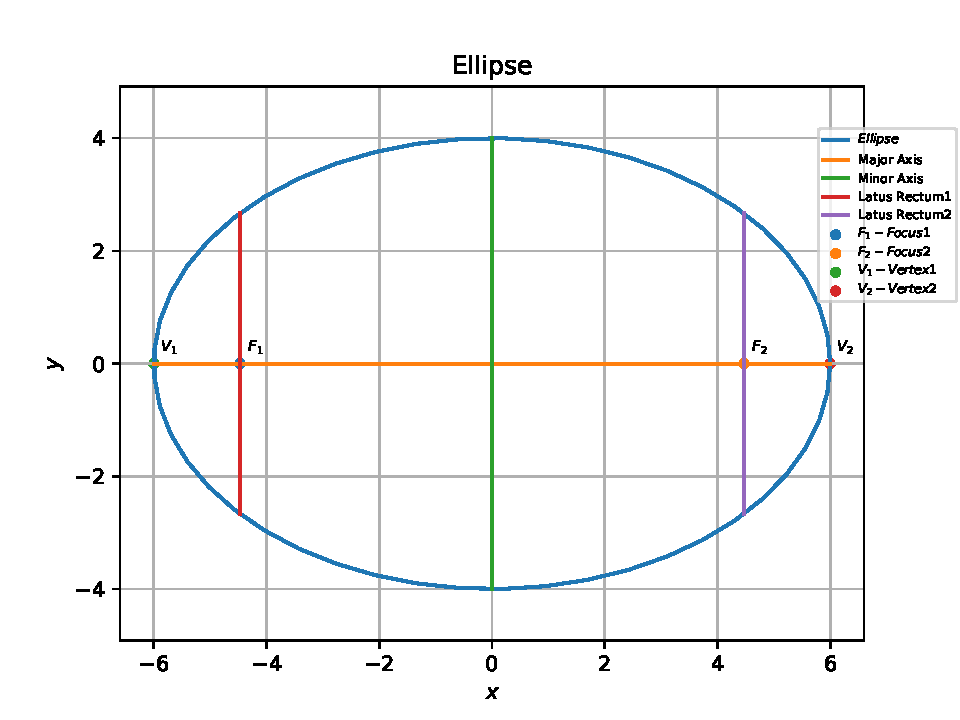
\includegraphics[width=\columnwidth]{chapters/11/11/3/1/figs/problem1.pdf}
	\end{center}
\caption{}
\label{fig:chapters/11/11/3/1/Fig1}
\end{figure}
\end{enumerate}

  \item $\frac{x^2}{4}+\frac{y^2}{25}=1$
\\
\solution
\iffalse
\documentclass[12pt]{article}
\usepackage{graphicx}
\usepackage{amsmath}
\usepackage{mathtools}
\usepackage{gensymb}

\newcommand{\mydet}[1]{\ensuremath{\begin{vmatrix}#1\end{vmatrix}}}
\providecommand{\brak}[1]{\ensuremath{\left(#1\right)}}
\providecommand{\norm}[1]{\left\lVert#1\right\rVert}
\providecommand{\abs}[1]{\left\vert#1\right\vert}
\newcommand{\solution}{\noindent \textbf{Solution: }}
\newcommand{\myvec}[1]{\ensuremath{\begin{pmatrix}#1\end{pmatrix}}}
\let\vec\mathbf

\begin{document}
\begin{center}
\textbf\large{CONIC SECTIONS}

\end{center}
\section*{Excercise 11.3}
Q2.Find the coordinates of the focii, the vertices, the length of major and minor axes, the eccentricity and the length of the latus rectum of an ellipse whose equation is given by $\frac{x^2}{4}+\frac{y^2}{25}=1$.

\solution
\fi
The equation of the given ellipse can be rearranged as 
\begin{align}
	\label{eq:chapters/11/11/3/2/eq1}
	25x^2+4y^2-100=0
\end{align}
The above equation can be equated to the generic equation of conic sections
\begin{align}
	\label{eq:chapters/11/11/3/2/eq2}
	g\brak{\vec{x}}=\vec{x}^\top \vec{V} \vec{x} + 2\vec{u}^\top \vec{x} + f = 0
\end{align}
Comparing coefficients of both equations \eqref{eq:chapters/11/11/3/2/eq1} and \eqref{eq:chapters/11/11/3/2/eq2}
\begin{align}
	\label{eq:chapters/11/11/3/2/eq3}
	\vec{V} &= \myvec{25&0\\0&4}\\
	\vec{u} &= \vec{0}\\
	f &= -100
\end{align}
From equation \eqref{eq:chapters/11/11/3/2/eq3}, since $\vec{V}$ is already diagonalized, the eigen values $\lambda_1 \text{ and } \lambda_2$ are given as
\begin{align}
	\lambda_1 &= 25\\
	\lambda_2 &= 4
\end{align}
Since the given matrix $\vec{V}$ is diagonal, the Eigen vector matrix will be identity. It is given as
\begin{align}
	\vec{P} &= \myvec{\vec{p}_1 & \vec{p}_2}\\
		&= \myvec{1&0\\0&1}
\end{align}
\begin{enumerate}
\item The eccentricity of the ellipse is given as
\begin{align}
	e &= \sqrt{1 - \frac{\lambda_2}{\lambda_1}} = \sqrt{1-\frac{4}{25}}\\
	  &= \frac{\sqrt{21}}{5}
\end{align}
\item Finding the coordinates of Focii
\begin{align}
	\vec{n} &= \sqrt{\lambda_1}\vec{p}_2= \sqrt{25} \myvec{0\\1}\\
	&= \myvec{0\\5}
\end{align}
\begin{align}
	\label{eq:chapters/11/11/3/2/eq4}
	c &= \frac{e\vec{u}^\top \vec{n} \pm \sqrt{e^2 \brak{\vec{u}^\top \vec{n}}^2-\lambda_1 \brak{e^2 -1}\brak{\norm{\vec{u}}^2-\lambda_1 f}}}{\lambda_1 e\brak{e^2-1}}
\end{align}
Substituting values of $e,\vec{u},\vec{n},\lambda_1 \text{ and } f$ in \eqref{eq:chapters/11/11/3/2/eq4}
\begin{align}
	c &= \frac{0 \pm \sqrt{0-25\brak{\frac{21}{25}-1}\brak{0+25\brak{100}}}}{25\frac{\sqrt{21}}{5}\brak{\frac{21}{25}-1}}\\
	&= \frac{\pm 125}{\sqrt{21}}
\end{align}
The focus $\vec{F}$ of the ellipse is expressed as
\begin{align}
	\vec{F} &= \frac{ce^2 \vec{n}-\vec{u}}{\lambda_1}\\
	&= \frac{\pm \frac{125}{\sqrt{21}}\brak{\frac{21}{25}}\myvec{0\\5}}{25}\\
	&= \myvec{0\\\pm \sqrt{21}}
\end{align}
\item The length of the major axis is given by
\begin{align}
	\label{eq:chapters/11/11/3/2/eq5}
	&2\sqrt{\abs{\frac{f_0}{\lambda_2}}}\\
	f_0 &= \vec{u}^\top \vec{V}^{-1} \vec{u} -f\\
	    &= 100\\
	\eqref{eq:chapters/11/11/3/2/eq5} &\implies 2\sqrt{\abs{\frac{100}{4}}}
	 = 10
\end{align}
\item The length of minor axis is given by
\begin{align}
	2\sqrt{\abs{\frac{f_0}{\lambda_1}}}&= 2\sqrt{\abs{\frac{100}{25}}}\\
	&= 4
\end{align}
\item The vertices of the ellipse are given by
\begin{align}
	\pm \myvec{0\\\sqrt{\abs{\frac{f_0}{\lambda_2}}}}= \pm \myvec{0\\5}
\end{align}
\item The length of latus rectum is given as
\begin{align}
	2\frac{\sqrt{\abs{f_0 \lambda_2}}}{\lambda_1} &= 2\frac{\sqrt{\abs{100\brak{4}}}}{25}\\
	&= \frac{8}{5}
\end{align}
\end{enumerate}
The corresponding is shown in Fig. \ref{fig:chapters/11/11/3/2/Fig1}.
\begin{figure}[!h]
	\begin{center} 
	    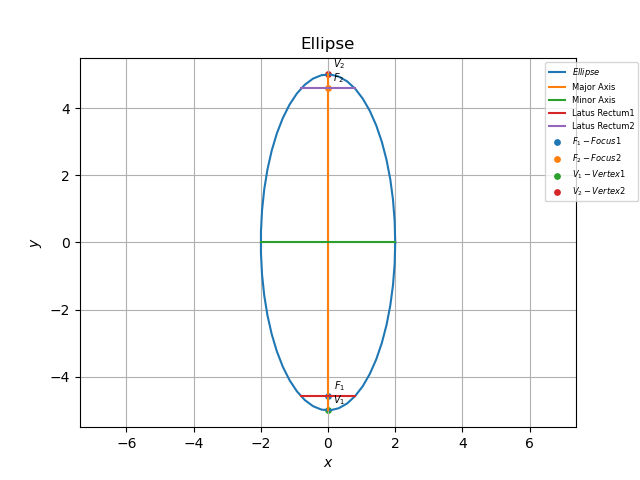
\includegraphics[width=\columnwidth]{chapters/11/11/3/2/figs/ellipse}
	\end{center}
\caption{}
\label{fig:chapters/11/11/3/2/Fig1}
\end{figure}

  \item $\frac{x^2}{16}+\frac{y^2}{9}=1$
\\
\solution
\iffalse
\documentclass[12pt]{article}
\usepackage{graphicx}
\usepackage[none]{hyphenat}
\usepackage{graphicx}
\usepackage{listings}
\usepackage[english]{babel}
\usepackage{graphicx}
\usepackage{caption} 
\usepackage{booktabs}
\usepackage{array}
\usepackage{amssymb} % for \because
\usepackage{amsmath}   % for having text in math mode
\usepackage{extarrows} % for Row operations arrows
\usepackage{listings}
\lstset{
  frame=single,
  breaklines=true
}
\usepackage{hyperref}
  
%Following 2 lines were added to remove the blank page at the beginning
\usepackage{atbegshi}% http://ctan.org/pkg/atbegshi
\AtBeginDocument{\AtBeginShipoutNext{\AtBeginShipoutDiscard}}


%New macro definitions
\newcommand{\mydet}[1]{\ensuremath{\begin{vmatrix}#1\end{vmatrix}}}
\providecommand{\brak}[1]{\ensuremath{\left(#1\right)}}
\providecommand{\norm}[1]{\left\lVert#1\right\rVert}
\providecommand{\abs}[1]{\left\vert#1\right\vert}
\newcommand{\solution}{\noindent \textbf{Solution: }}
\newcommand{\myvec}[1]{\ensuremath{\begin{pmatrix}#1\end{pmatrix}}}
\let\vec\mathbf


\begin{document}

\begin{center}
\title{\textbf{Conic Sections - Ellipse}}
\date{\vspace{-5ex}} %Not to print date automatically
\maketitle
\end{center}
\setcounter{page}{1}

\section{11$^{th}$ Maths - Chapter 11}
This is Problem-3 from Exercise 11.3
\begin{enumerate}
\item Find the coordinates of the focii, the vertices, the length of major and minor axes, the eccentricity and the length of the latus rectum of an ellipse whose equation is given by $\frac{x^2}{16}+\frac{y^2}{9}=1$.

\solution
\fi
The given equation of ellipse can be rearranged as 
\begin{align}
 9x^2+16y^2-144=0\label{eq:chapters/11/11/3/3/eq1}
\end{align}
The above equation can be equated to the general equation of conic sections
\begin{align}
 g\brak{\vec{x}}=\vec{x}^\top \vec{V} \vec{x} + 2\vec{u}^\top \vec{x} + f = 0\label{eq:chapters/11/11/3/3/eq2}
\end{align}
From \eqref{eq:chapters/11/11/3/3/eq1} and \eqref{eq:chapters/11/11/3/3/eq2}
\begin{align}
 \vec{V} &= \myvec{9&0\\0&16}\label{eq:chapters/11/11/3/3/eq3}\\
 \vec{u} &= \vec{0}\\
 f &= -144
\end{align}
From \eqref{eq:chapters/11/11/3/3/eq3} the eigen values $\lambda_1 \text{ and } \lambda_2$ are given as
\begin{align}
 \lambda_1 &= 9\\
 \lambda_2 &= 16
\end{align}
\begin{enumerate}
\item The eccentricity of the ellipse is given as
\begin{align}
 e &= \sqrt{1 - \frac{\lambda_2}{\lambda_1}} \\
          &= \sqrt{1-\frac{9}{16}}\\
   &= \frac{\sqrt{7}}{4}
\end{align}
\item Finding the coordinates of Focii
\begin{align}
 \vec{F} &= \pm e\sqrt{\frac{\abs{f_0}}{\lambda_2\brak{1-e^2}}}\Vec{e_1}\\
\text{Where }f_0 &=-f\\
 \vec{F} &= \pm\sqrt{7}\myvec{1\\0}\\
	&= \pm\myvec{\sqrt{7}\\0}
\end{align}
\item The length of the major axis is given by
\begin{align}
 &2\sqrt{\abs{\frac{f_0}{\lambda_1}}}\\
        &2\sqrt{\abs{\frac{144}{9}}}= 8
\end{align}
\item The length of minor axis is given by
\begin{align}
 &2\sqrt{\abs{\frac{f_0}{\lambda_2}}}\\
        &2\sqrt{\abs{\frac{144}{16}}}= 6
\end{align}
\item The vertices of the ellipse are given by
\begin{align}
 \pm \myvec{0\\\sqrt{\abs{\frac{f_0}{\lambda_2}}}}= \pm \myvec{0\\4}
\end{align}
\item The length of latus rectum is given as
\begin{align}
 &2\frac{\sqrt{\abs{f_0 \lambda_1}}}{\lambda_2} \\
 &= 2\frac{\sqrt{\abs{144\brak{9}}}}{16}\\
 &= \frac{9}{2}
\end{align}
\begin{figure}[!h]
	\begin{center}
		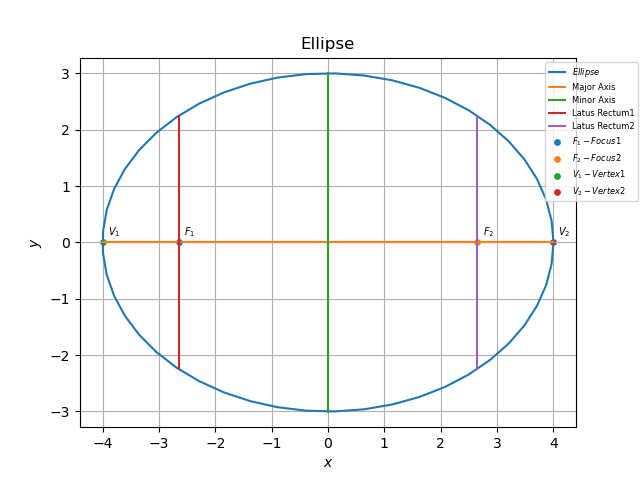
\includegraphics[width=\columnwidth]{chapters/11/11/3/3/figs/conic.png}
	\end{center}
\caption{}
\label{fig:chapters/11/11/3/3/Fig1}
\end{figure}
\end{enumerate}

  \item $\frac{x^2}{25}+\frac{y^2}{100}=1$
  \item $\frac{x^2}{49}+\frac{y^2}{36}=1$
  \item $\frac{x^2}{100}+\frac{y^2}{400}=1$
  \item $36x^2+4y^2=144$
  \item $16x^2+y^2=16$
  \item $4x^2+9y^2=36$
\end{enumerate}

In each of the following exercises,  find the equation for the ellipse that satisfies the given conditions

%\begin{enumerate}[label=\thesection.\arabic*,ref=\thesection.\theenumi][resume]
\begin{enumerate}[resume*]
\item vertices $(\pm5,0),\text{foci} (\pm4,0)$
\item vertices $(\pm0,13),\text{foci} (0,\pm5)$
\item vertices $(\pm6,0),\text{foci} (\pm4,0)$
\item Ends of major axis $(\pm3,0),\text{ends of minor axis}(0,\pm2)$
\item  ends of major axis $(0,\pm \sqrt{5}),\text{ends of minor axis} (\pm1,0)$
\item $\text {length of major axis 26},\text{foci} (\pm5,0)$
\item $\text {length of minor axis 16},\text{foci} (0,\pm6)$
\item $\text {foci} (\pm3,0),a=4$
\item $\text {b=3,c=4},\text {centre at the origin} ;\text{foci on the x axis}$
\item $\text {centre at} (0,0),\text{major axis on the y-axis and passes through the points} \text {(3,2) and (1,6)}$.
\\
\solution
\iffalse
\documentclass[journal,12pt,twocolumn]{IEEEtran}
\usepackage{setspace}
\usepackage{gensymb}
\singlespacing
\usepackage[cmex10]{amsmath}
\usepackage{amsthm}
\usepackage{mathrsfs}
\usepackage{txfonts}
\usepackage{stfloats}
\usepackage{bm}
\usepackage{cite}
\usepackage{cases}
\usepackage{subfig}
\usepackage{longtable}
\usepackage{multirow}
\usepackage{enumitem}
\usepackage{mathtools}
\usepackage{steinmetz}
\usepackage{tikz}
\usepackage{circuitikz}
\usepackage{verbatim}
\usepackage{tfrupee}
\usepackage[breaklinks=true]{hyperref}
\usepackage{tkz-euclide}
\usetikzlibrary{calc,math}
\usepackage{listings}
    \usepackage{color}                                            %%
    \usepackage{array}                                            %%
    \usepackage{longtable}                                        %%
    \usepackage{calc}                                             %%
    \usepackage{multirow}                                         %%
    \usepackage{hhline}                                           %%
    \usepackage{ifthen}                                           %%
  %optionally (for landscape tables embedded in another document): %%
    \usepackage{lscape}     
\usepackage{multicol}
\usepackage{chngcntr}
\DeclareMathOperator*{\Res}{Res}
\renewcommand\thesection{\arabic{section}}
\renewcommand\thesubsection{\thesection.\arabic{subsection}}
\renewcommand\thesubsubsection{\thesubsection.\arabic{subsubsection}}

\renewcommand\thesectiondis{\arabic{section}}
\renewcommand\thesubsectiondis{\thesectiondis.\arabic{subsection}}
\renewcommand\thesubsubsectiondis{\thesubsectiondis.\arabic{subsubsection}}

% correct bad hyphenation here
\hyphenation{op-tical net-works semi-conduc-tor}
\def\inputGnumericTable{}                                 %%

\lstset{
frame=single, 
breaklines=true,
columns=fullflexible
}

\begin{document}


\newtheorem{theorem}{Theorem}[section]
\newtheorem{problem}{Problem}
\newtheorem{proposition}{Proposition}[section]
\newtheorem{lemma}{Lemma}[section]
\newtheorem{corollary}[theorem]{Corollary}
\newtheorem{example}{Example}[section]
\newtheorem{definition}[problem]{Definition}
\newcommand{\BEQA}{\begin{eqnarray}}
\newcommand{\EEQA}{\end{eqnarray}}
\newcommand{\define}{\stackrel{\triangle}{=}}

\bibliographystyle{IEEEtran}
\providecommand{\mbf}{\mathbf}
\providecommand{\pr}[1]{\ensuremath{\Pr\left(#1\right)}}
\providecommand{\qfunc}[1]{\ensuremath{Q\left(#1\right)}}
\providecommand{\sbrak}[1]{\ensuremath{{}\left[#1\right]}}
\providecommand{\lsbrak}[1]{\ensuremath{{}\left[#1\right.}}
\providecommand{\rsbrak}[1]{\ensuremath{{}\left.#1\right]}}
\providecommand{\brak}[1]{\ensuremath{\left(#1\right)}}
\providecommand{\lbrak}[1]{\ensuremath{\left(#1\right.}}
\providecommand{\rbrak}[1]{\ensuremath{\left.#1\right)}}
\providecommand{\cbrak}[1]{\ensuremath{\left\{#1\right\}}}
\providecommand{\lcbrak}[1]{\ensuremath{\left\{#1\right.}}
\providecommand{\rcbrak}[1]{\ensuremath{\left.#1\right\}}}
\theoremstyle{remark}
\newtheorem{rem}{Remark}
\newcommand{\sgn}{\mathop{\mathrm{sgn}}}
\providecommand{\abs}[1]{\left\vert#1\right\vert}
\providecommand{\res}[1]{\Res\displaylimits_{#1}} 
\providecommand{\norm}[1]{\left\lVert#1\right\rVert}
\providecommand{\mtx}[1]{\mathbf{#1}}
\providecommand{\mean}[1]{E\left[ #1 \right]}
\providecommand{\fourier}{\overset{\mathcal{F}}{ \rightleftharpoons}}
\providecommand{\system}{\overset{\mathcal{H}}{ \longleftrightarrow}}
\newcommand{\solution}{\noindent \textbf{Solution: }}
\newcommand{\cosec}{\,\text{cosec}\,}
\providecommand{\dec}[2]{\ensuremath{\overset{#1}{\underset{#2}{\gtrless}}}}
\newcommand{\myvec}[1]{\ensuremath{\begin{pmatrix}#1\end{pmatrix}}}
\newcommand{\mydet}[1]{\ensuremath{\begin{vmatrix}#1\end{vmatrix}}}
\numberwithin{equation}{subsection}
\makeatletter
\@addtoreset{figure}{problem}
\makeatother

\let\StandardTheFigure\thefigure
\let\vec\mathbf
\renewcommand{\thefigure}{\theproblem}



\def\putbox#1#2#3{\makebox[0in][l]{\makebox[#1][l]{}\raisebox{\baselineskip}[0in][0in]{\raisebox{#2}[0in][0in]{#3}}}}
     \def\rightbox#1{\makebox[0in][r]{#1}}
     \def\centbox#1{\makebox[0in]{#1}}
     \def\topbox#1{\raisebox{-\baselineskip}[0in][0in]{#1}}
     \def\midbox#1{\raisebox{-0.5\baselineskip}[0in][0in]{#1}}

\vspace{3cm}


\title{Assignment 1}
\author{Jaswanth Chowdary Madala}





% make the title area
\maketitle

\newpage

%\tableofcontents

\bigskip

\renewcommand{\thefigure}{\theenumi}
\renewcommand{\thetable}{\theenumi}


\begin{enumerate}
\item Find the equation of the ellipse that satisfies the conditions - Centre at $\brak{0,0}$, major axis on the y-axis and passes through the points $\brak{3,2}$ and $\brak{1,6}$.
%\begin{figure}[ht]
%\centering
%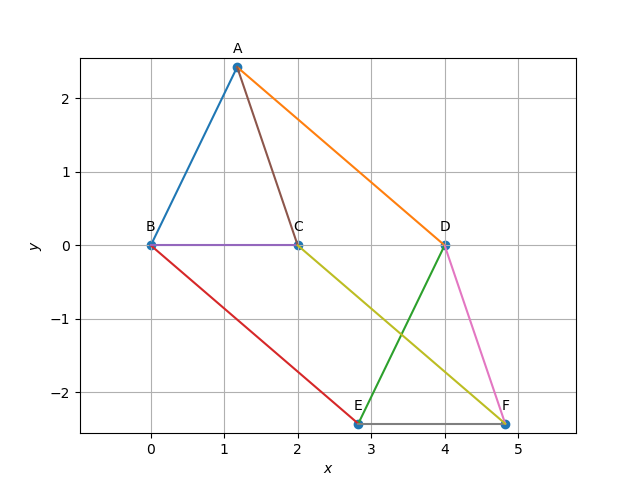
\includegraphics[width = \columnwidth]{"./chapters/11/11/3/19/figs/fig.png"}
%\caption{Graph}
%\label{fig:chapters/11/11/3/19/1}
%\end{figure}

\textbf{Solution:}
\fi
The input parameters are listed in 
\ref{tab:chapters/11/11/3/19/1}.
The equation of the conic with focus $\vec{F}$, directrix $\vec{n}^\top\vec{x} = c$ and eccentricity $e$ is given by
\begin{align}
\vec{x}^\top\vec{V}\vec{x} + 2\vec{u}^\top\vec{x} + f = 0
\label{eq:chapters/11/11/3/19/1}
\end{align}
where
\begin{align}
\vec{V} &\triangleq \norm{\vec{n}}^2\vec{I} - e^2\vec{n}\vec{n}^\top \label{eq:chapters/11/11/3/19/2} \\
\vec{u} &\triangleq ce^2\vec{n} - \norm{\vec{n}}^2\vec{F} \label{eq:chapters/11/11/3/19/3} \\
f &\triangleq \norm{\vec{n}}^2\norm{\vec{F}}^2 - c^2e^2 \label{eq:chapters/11/11/3/19/4}
\end{align}
Given that the conic is an ellipse with major axis along the $y$-axis,
\begin{align}
\vec{n} = \myvec{0\\1}
\end{align}
Thus,
\begin{align}
\vec{V} = \myvec{1&0\\0&1-e^2} \label{eq:chapters/11/11/3/19/5} \\
\vec{u} = ce^2\myvec{0\\1} - \vec{F} \label{eq:chapters/11/11/3/19/6} \\
f = \norm{\vec{F}}^2 - c^2e^2 \label{eq:chapters/11/11/3/19/7}
\end{align}
The centre of the conic is given by
\begin{align}
\vec{c} = -\vec{V}^{-1}\vec{u}
\label{eq:chapters/11/11/3/19/8}
\end{align}
Since $\vec{c} = \vec{0}$ and $\vec{V}^{-1} \neq \vec{0}$, it follows from \eqref{eq:chapters/11/11/3/19/8} that 
\begin{align}
\vec{u} = \vec{0}
\end{align}
Thus, from \eqref{eq:chapters/11/11/3/19/6},
\begin{align}
\vec{F} = \myvec{0\\ce^2}
\label{eq:chapters/11/11/3/19/9}
\end{align}
and so,
\begin{align}
f = c^2e^2\brak{e^2-1}
%\label{eq:chapters/11/11/3/19/9}
\end{align}
Given that the conic passes through 
\begin{align}
\vec{P} = \myvec{3\\2},
\end{align}
putting $\vec{x} = \vec{P}$ in \eqref{eq:chapters/11/11/3/19/1} we get,
\begin{align}
\myvec{3&2}\myvec{1&0\\0&1-e^2}\myvec{3\\2} + f &= 0 \\
\implies 4e^2 - f = 13 \label{eq:chapters/11/11/3/19/10}
\end{align}
Given that the conic passes through
\begin{align}
\vec{Q} = \myvec{1\\6},
\end{align}
putting $\vec{x} = \vec{Q}$ in \eqref{eq:chapters/11/11/3/19/1}, we get
\begin{align}
\myvec{1&6}\myvec{1&0\\0&1-e^2}\myvec{1\\6} + f &= 0 \\
\implies 36e^2 - f = 37 \label{eq:chapters/11/11/3/19/11}
\end{align}
The equations \eqref{eq:chapters/11/11/3/19/10} and \eqref{eq:chapters/11/11/3/19/11} can be formulated as the following matrix equation
\begin{align}
\myvec{4&-1\\36&-1}\myvec{e^2\\f} = \myvec{13\\37}
\label{eq:chapters/11/11/3/19/12}
\end{align}
The augmented matrix is given by,
\begin{align}
\myvec{4&-1&\vline&13\\36&-1&\vline&37}
\end{align}
yielding
\begin{align}
\xleftrightarrow[]{R_1\leftarrow R_1-R_2} &\myvec{-32&0&\vline&-24\\36&-1&\vline&37} \\
\xleftrightarrow[]{R_1\leftarrow-\frac{R_1}{8}}& \myvec{4&0&\vline&3\\36&-1&\vline&37} \\
\xleftrightarrow[]{R_2\leftarrow R_2-9R_1}
&\myvec{4&0&\vline&3\\0&-1&\vline&10} \\
\xleftrightarrow[R_2\leftarrow -R_2]{R_1\leftarrow \frac{R_1}{4}}
&\myvec{1&0&\vline&\frac{3}{4}\\0&1&\vline&-10}
\end{align}
Thus,
\begin{align}
e^2 = \frac{3}{4},\ f = -10
\end{align}
and the equation of the conic is given by
\begin{align}
\vec{x}^\top\myvec{1&0\\0&\frac{1}{4}}\vec{x} - 10 = 0
\end{align}
See Fig. 
\ref{fig:chapters/11/11/3/19/1}.
\begin{figure}[ht]
\centering
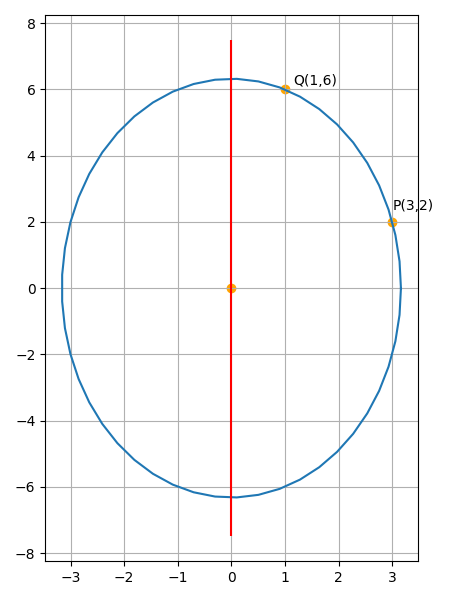
\includegraphics[width = \columnwidth]{chapters/11/11/3/19/figs/fig1.png}
\caption{Graph}
\label{fig:chapters/11/11/3/19/1}
\end{figure}
\begin{table}[h]
\centering
%%%%%%%%%%%%%%%%%%%%%%%%%%%%%%%%%%%%%%%%%%%%%%%%%%%%%%%%%%%%%%%%%%%%%%
%%                                                                  %%
%%  This is a LaTeX2e table fragment exported from Gnumeric.        %%
%%                                                                  %%
%%%%%%%%%%%%%%%%%%%%%%%%%%%%%%%%%%%%%%%%%%%%%%%%%%%%%%%%%%%%%%%%%%%%%%

\begin{center}
\begin{tabular}{|c|c|c|}
\hline
\textbf{Parameter}& \textbf{Description} &\textbf{Value}\\ \hline
$\vec{C}$		 &	center of the ellipse&$\myvec{0\\0}$\\ \hline
$\vec{m}$		 &	Direction vector of major axis &$\myvec{0\\1}$\\ \hline
$\vec{P}$		 &  Point on the ellipse&$\myvec{3\\2}$ \\ \hline
$\vec{Q}$		 &  Point on the ellipse&$\myvec{1\\6}$ \\ \hline
\end{tabular}
\end{center}

\caption{}
\label{tab:chapters/11/11/3/19/1}
\end{table}

\item $\text{major axis on the x-axis and passes through the points (4,3) and (6,2)}$
\\
\solution
\iffalse
\documentclass[journal,12pt,twocolumn]{IEEEtran}
\usepackage{setspace}
\usepackage{gensymb}
\usepackage{xcolor}
\usepackage{caption}
\singlespacing
\usepackage{siunitx}
\usepackage[cmex10]{amsmath}
\usepackage{mathtools}
\usepackage{hyperref}
\usepackage{amsthm}
\usepackage{mathrsfs}
\usepackage{txfonts}
\usepackage{stfloats}
\usepackage{cite}
\usepackage{cases}
\usepackage{subfig}
\usepackage{longtable}
\usepackage{multirow}
\usepackage{enumitem}
\usepackage{bm}
\usepackage{mathtools}
\usepackage{listings}
\usepackage{tikz}
\usetikzlibrary{shapes,arrows,positioning}
\usepackage{circuitikz}
\renewcommand{\vec}[1]{\boldsymbol{\mathbf{#1}}}
\DeclareMathOperator*{\Res}{Res}
\renewcommand\thesection{\arabic{section}}
\renewcommand\thesubsection{\thesection.\arabic{subsection}}
\renewcommand\thesubsubsection{\thesubsection.\arabic{subsubsection}}

\renewcommand\thesectiondis{\arabic{section}}
\renewcommand\thesubsectiondis{\thesectiondis.\arabic{subsection}}
\renewcommand\thesubsubsectiondis{\thesubsectiondis.\arabic{subsubsection}}
\hyphenation{op-tical net-works semi-conduc-tor}

\lstset{
language=Python,
frame=single, 
breaklines=true,
columns=fullflexible
}
\begin{document}
\theoremstyle{definition}
\newtheorem{theorem}{Theorem}[section]
\newtheorem{problem}{Problem}
\newtheorem{proposition}{Proposition}[section]
\newtheorem{lemma}{Lemma}[section]
\newtheorem{corollary}[theorem]{Corollary}
\newtheorem{example}{Example}[section]
\newtheorem{definition}{Definition}[section]
\newcommand{\BEQA}{\begin{eqnarray}}
\newcommand{\EEQA}{\end{eqnarray}}
\newcommand{\define}{\stackrel{\triangle}{=}}
\newcommand{\myvec}[1]{\ensuremath{\begin{pmatrix}#1\end{pmatrix}}}
\newcommand{\mydet}[1]{\ensuremath{\begin{vmatrix}#1\end{vmatrix}}}
\bibliographystyle{IEEEtran}
\providecommand{\nCr}[2]{\,^{#1}C_{#2}} % nCr
\providecommand{\nPr}[2]{\,^{#1}P_{#2}} % nPr
\providecommand{\mbf}{\mathbf}
\providecommand{\pr}[1]{\ensuremath{\Pr\left(#1\right)}}
\providecommand{\qfunc}[1]{\ensuremath{Q\left(#1\right)}}
\providecommand{\sbrak}[1]{\ensuremath{{}\left[#1\right]}}
\providecommand{\lsbrak}[1]{\ensuremath{{}\left[#1\right.}}
\providecommand{\rsbrak}[1]{\ensuremath{{}\left.#1\right]}}
\providecommand{\brak}[1]{\ensuremath{\left(#1\right)}}
\providecommand{\lbrak}[1]{\ensuremath{\left(#1\right.}}
\providecommand{\rbrak}[1]{\ensuremath{\left.#1\right)}}
\providecommand{\cbrak}[1]{\ensuremath{\left\{#1\right\}}}
\providecommand{\lcbrak}[1]{\ensuremath{\left\{#1\right.}}
\providecommand{\rcbrak}[1]{\ensuremath{\left.#1\right\}}}
\theoremstyle{remark}
\newtheorem{rem}{Remark}
\newcommand{\sgn}{\mathop{\mathrm{sgn}}}
\newcommand{\rect}{\mathop{\mathrm{rect}}}
\newcommand{\sinc}{\mathop{\mathrm{sinc}}}
\providecommand{\abs}[1]{\left\vert#1\right\vert}
\providecommand{\res}[1]{\Res\displaylimits_{#1}} 
\providecommand{\norm}[1]{\lVert#1\rVert}
\providecommand{\mtx}[1]{\mathbf{#1}}
\providecommand{\mean}[1]{E\left[ #1 \right]}
\providecommand{\fourier}{\overset{\mathcal{F}}{ \rightleftharpoons}}
\providecommand{\ztrans}{\overset{\mathcal{Z}}{ \rightleftharpoons}}
\providecommand{\system}[1]{\overset{\mathcal{#1}}{ \longleftrightarrow}}
\newcommand{\solution}{\noindent \textbf{Solution: }}
\providecommand{\dec}[2]{\ensuremath{\overset{#1}{\underset{#2}{\gtrless}}}}
\let\StandardTheFigure\thefigure
\def\putbox#1#2#3{\makebox[0in][l]{\makebox[#1][l]{}\raisebox{\baselineskip}[0in][0in]{\raisebox{#2}[0in][0in]{#3}}}}
     \def\rightbox#1{\makebox[0in][r]{#1}}
     \def\centbox#1{\makebox[0in]{#1}}
     \def\topbox#1{\raisebox{-\baselineskip}[0in][0in]{#1}}
     \def\midbox#1{\raisebox{-0.5\baselineskip}[0in][0in]{#1}}

\vspace{3cm}
\title{Conic Assignment}
\author{Gautam Singh}
\maketitle
\bigskip

\begin{abstract}
    This document contains the solution to Question 20 of Exercise 3 in Chapter
    11 of the class 11 NCERT textbook.
\end{abstract}

\begin{enumerate}
    \item Find the equation of the ellipse whose major axis is the $x$-axis and
    center is the origin and passes through the points
    \begin{align}
        \vec{P} = \myvec{4\\3},\ \vec{Q} = \myvec{6\\2}
    \end{align}

    \solution 
\fi
		Let the equation of the conic with focus $\vec{F}$, directrix
    $\vec{n}^\top\vec{x} = c$ and eccentricity $e$ be
    \begin{align}
        \vec{x}^\top\vec{V}\vec{x} + 2\vec{u}^\top\vec{x} + f = 0
        \label{eq:chapters/11/11/3/20/conic-def}
    \end{align}
    where
    \begin{align}
        \vec{V} &\triangleq \norm{\vec{n}}^2\vec{I} - e^2\vec{n}\vec{n}^\top \label{eq:chapters/11/11/3/20/V-def} \\
        \vec{u} &\triangleq ce^2\vec{n} - \norm{\vec{n}}^2\vec{F} \label{eq:chapters/11/11/3/20/u-def} \\
        f &\triangleq \norm{\vec{n}}^2\norm{\vec{F}}^2 - c^2e^2 \label{eq:chapters/11/11/3/20/f-def}
    \end{align}
    Since the conic is an ellipse whose major axis is along the $x$-axis, we have
    \begin{align}
        \vec{n} = \myvec{1\\0}
    \end{align}
    Thus,
    \begin{align}
        \vec{V} = \myvec{1-e^2&0\\0&1} \label{eq:chapters/11/11/3/20/V-val} \\
        \vec{u} = ce^2\myvec{1\\0} - \vec{F} \label{eq:chapters/11/11/3/20/u-val} \\
        f = \norm{\vec{F}}^2 - c^2e^2 \label{eq:chapters/11/11/3/20/f-val}
    \end{align}
    The centre of the conic is given by
    \begin{align}
        \vec{c} = -\vec{V}^{-1}\vec{u}
        \label{eq:chapters/11/11/3/20/center}
    \end{align}
    Since $\vec{c} = \vec{0}$ and $\vec{V}^{-1} \neq \vec{0}$, it follows from 
    \eqref{eq:chapters/11/11/3/20/center} that $\vec{u} = \vec{0}$. Thus, from \eqref{eq:chapters/11/11/3/20/u-val},
    \begin{align}
        \vec{F} = \myvec{ce^2\\0}
        \label{eq:chapters/11/11/3/20/F-c-e}
    \end{align}
    and so,
    \begin{align}
        f = c^2e^2\brak{e^2-1}
        \label{eq:chapters/11/11/3/20/f-c-e}
    \end{align}
    Putting $\vec{x} = \vec{P}$ in \eqref{eq:chapters/11/11/3/20/conic-def} and using \eqref{eq:chapters/11/11/3/20/F-c-e}
    and \eqref{eq:chapters/11/11/3/20/f-c-e},
    \begin{align}
        \myvec{4&3}\myvec{1-e^2&0\\0&1}\myvec{4\\3} + f &= 0 \\
        \implies 16e^2 - f = 25 \label{eq:chapters/11/11/3/20/e1}
    \end{align}
    Putting $\vec{x} = \vec{Q}$ in \eqref{eq:chapters/11/11/3/20/conic-def}, we get
    \begin{align}
        \myvec{6&2}\myvec{1-e^2&0\\0&1}\myvec{6\\2} + f &= 0 \\
        \implies 36e^2 - f = 40 \label{eq:chapters/11/11/3/20/e2}
    \end{align}
    The equations \eqref{eq:chapters/11/11/3/20/e1} and \eqref{eq:chapters/11/11/3/20/e2} can be formulated as
    a matrix equation
    \begin{align}
        \myvec{16&-1\\36&-1}\myvec{e^2\\f} = \myvec{25\\40}
        \label{eq:chapters/11/11/3/20/mtx-eqn}
    \end{align}
    and can be solved using the augmented matrix.
    \begin{align}
        \myvec{16&-1&25\\36&-1&40} &\xleftrightarrow[]{R_1\leftarrow R_1-R_2} \myvec{-20&0&-15\\36&-1&40} \\
                 &\xleftrightarrow[]{\substack{R_1\leftarrow\frac{R_1}{-5}\\R_2\leftarrow -R_2}} \myvec{4&0&3\\-36&1&-40} \\
                 &\xleftrightarrow[]{R_2\leftarrow R_2+9R_1}\myvec{4&0&3\\0&1&-13} \\
                 &\xleftrightarrow[]{R_1\leftarrow\frac{R_1}{4}}\myvec{1&0&\frac{3}{4}\\0&1&-13}
    \end{align}
    Thus,
    \begin{align}
        e^2 = \frac{3}{4},\ f = -13
    \end{align}
    And the equation of the conic is given by
    \begin{align}
        \vec{x}^\top\myvec{\frac{1}{4}&0\\0&1}\vec{x} - 13 = 0
    \end{align}
    The situation is illustrated in Fig. \ref{fig:chapters/11/11/3/20/ellipse}
    \begin{figure}[!ht]
        \centering
        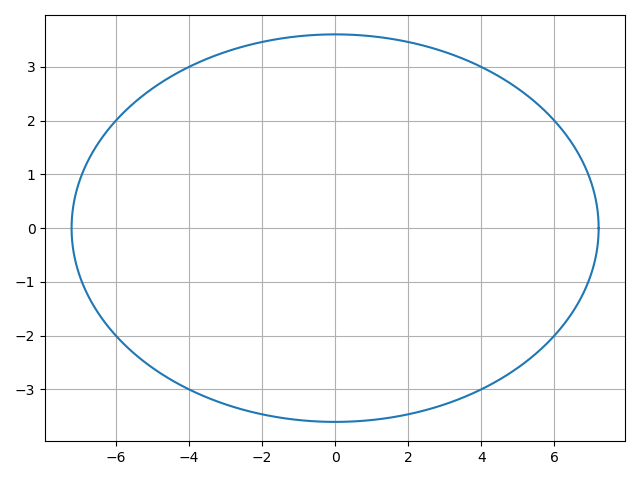
\includegraphics[width=\columnwidth]{chapters/11/11/3/20/figs/ellipse.png}
        \caption{Locus of the required ellipse.}
        \label{fig:chapters/11/11/3/20/ellipse}
    \end{figure}


\end{enumerate}
